%%%%%%%%%%%%%%%%%%%%%%%%%%%%%%%%%%%%%%%%%%%%%%%%%%%%%%%%%%%%%%%%%%%%%%%%%%%%%
%%% A Dependency Network+Weigthed Kernel Approach for Feature Selection
%%% Proposal for a MSc Project
%%% Nestor Rodriguez + Sergio A. Rojas (c) 2010
%%%
%%% Chapter 3: Acknowledgements
%%%%%%%%%%%%%%%%%%%%%%%%%%%%%%%%%%%%%%%%%%%%%%%%%%%%%%%%%%%%%%%%%%%%%%%%%%%%%

\pdfcomment[avatar={reviewer}, id=3]{I would expect a precisely established methodology along with a list of planned activities and their expected execution times.}
\pdfreply[avatar=me, id=30, replyto=3]{Two new sections were created as an answer to your recommendations.  The One represents the methodology, and the other, named 'Timeline', represents the planned activities with their expected execution times.}
\section{Methodology}
This section explains the intended methodology for this thesis.

\subsection{Literature Review}
In this stage a review of the state-of-the-art in population-based stochastic search methods for feature selection, estimation of dependency networks and weighted kernel classifiers will be carried out. The outcome of this stage will be a literature review report.

\subsection{Algorithm Design}
In this stage we will study in detail the elements described in Figure \ref{fig:im02}, \ref{fig:im03}, and Algorithm \ref{alg:idea} in order to provide the final design of the proposed method, according to the goals stated in Section \ref{sec:goals}.  

\subsection{Algorithm Implementation}
In this stage we will choose the development tools (programming language and developing environment, source code management) and carry out the implementation of the algorithm, along with its documentation and a supporting website. The outcome of this stage will be a ready-to-use computer program.

\subsection{Experimentation}
In this stage we will test the program using toy and real datasets in controlled conditions. We will also compare its performance with other feature selection techniques. The experiments will involve the following tasks:
\begin{enumerate}
	\item Dataset preparation:  This task comprises the creation of synthetic tabular datasets with different testing properties (number of dimensions, variable dependencies, linear or non-linear concepts, etc) and search and preparation of real problem datasets.
	\item Experimental design:  This task comprises the design of different scenarios and hypothesis to test (input parameters, performance measures, etc.). 
	\item Experiments execution:  This task comprises setting up the experimental platform, implementation of required algorithms, running up the designed experiments and collections of results in a suitable form for interpretations (tables, figures, etc.).
\end{enumerate}

\subsection{Analysis of Results}
In this stage the results obtained in the previous stages will be analyzed and the the feasibility of the algorithm will be discussed in view of the proposed research hypothesis and goals.

\subsection{Conclusions and Documentation}
This stage involves writing up the final technical report including conclusions and views derived from the research work that was conducted and recommendations for future work.

\clearpage
%\begin{landscape}
\section{Timeline}
\label{sec:TheSch}
\begin{figure}[h]
	\centering
		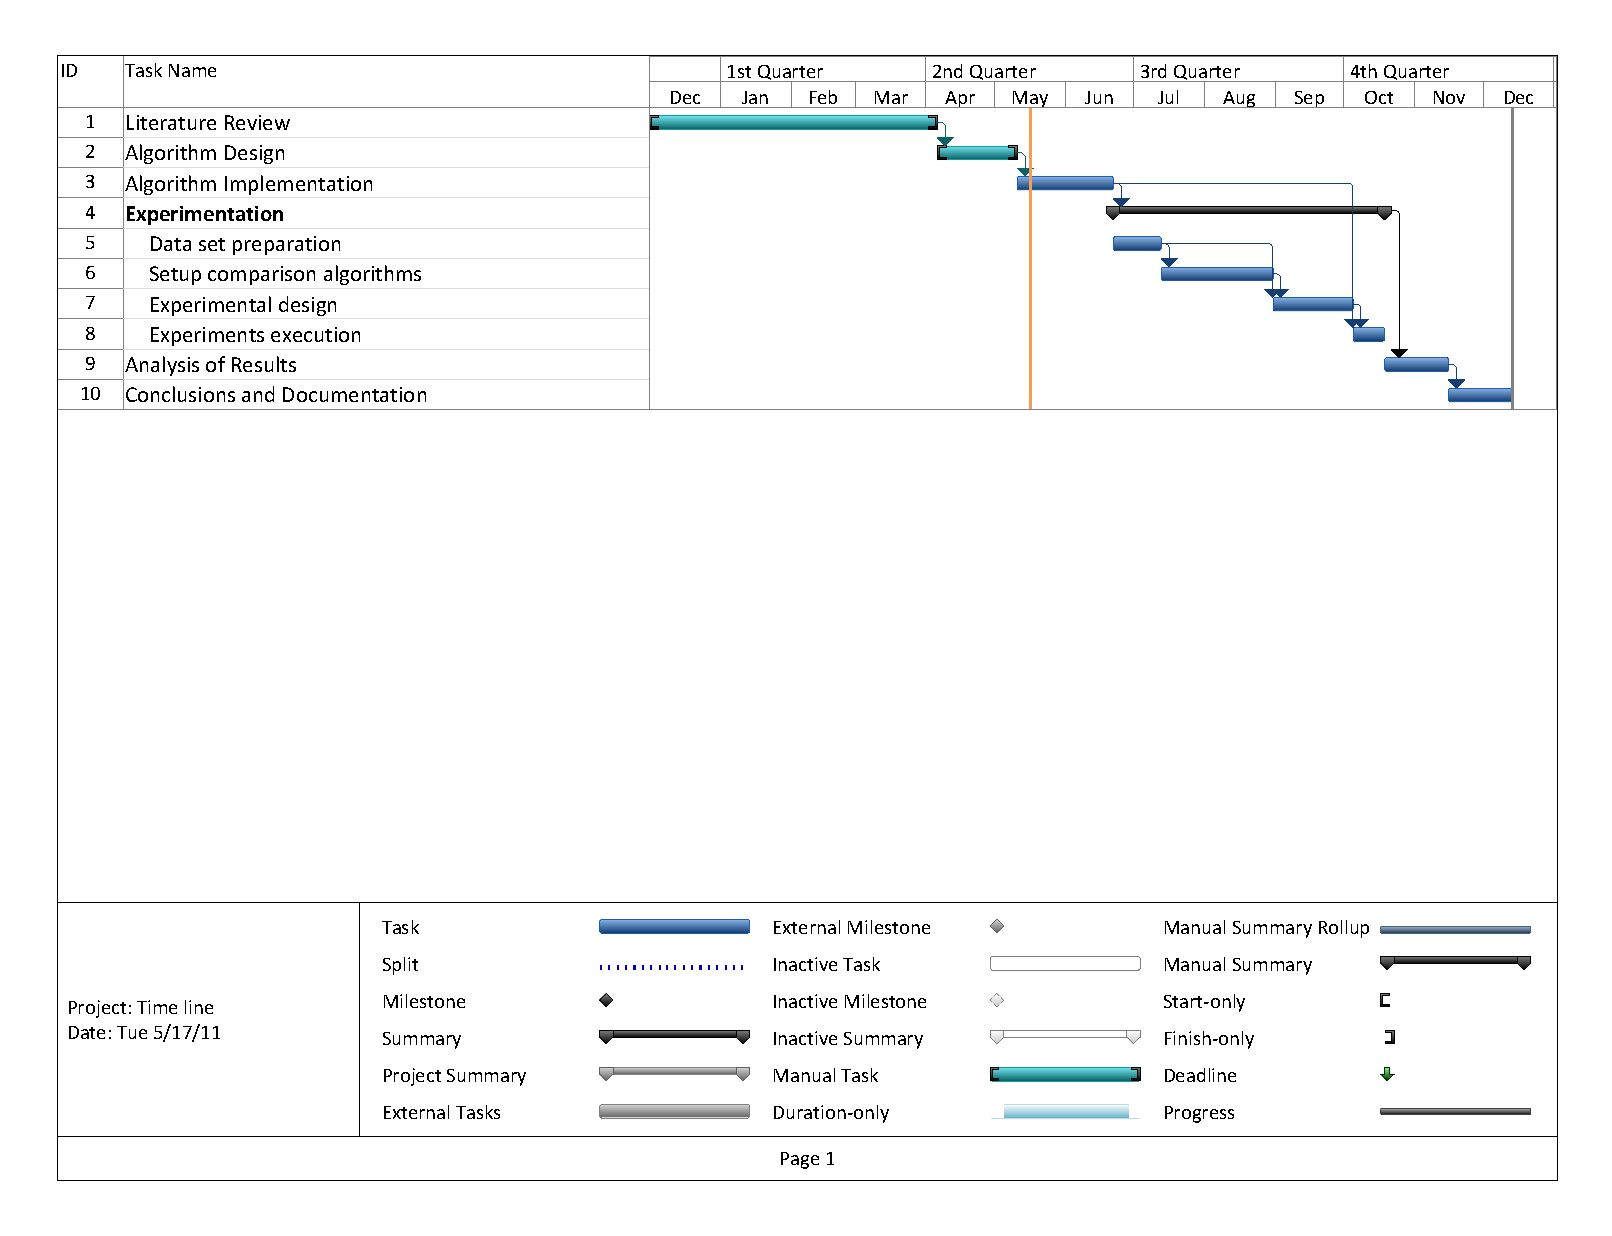
\includegraphics[scale=0.5]{Images/Timeline.pdf}
	\caption{Timeline for the thesis proposal.}
	\label{fig:sche}
\end{figure}
%\end{landscape}